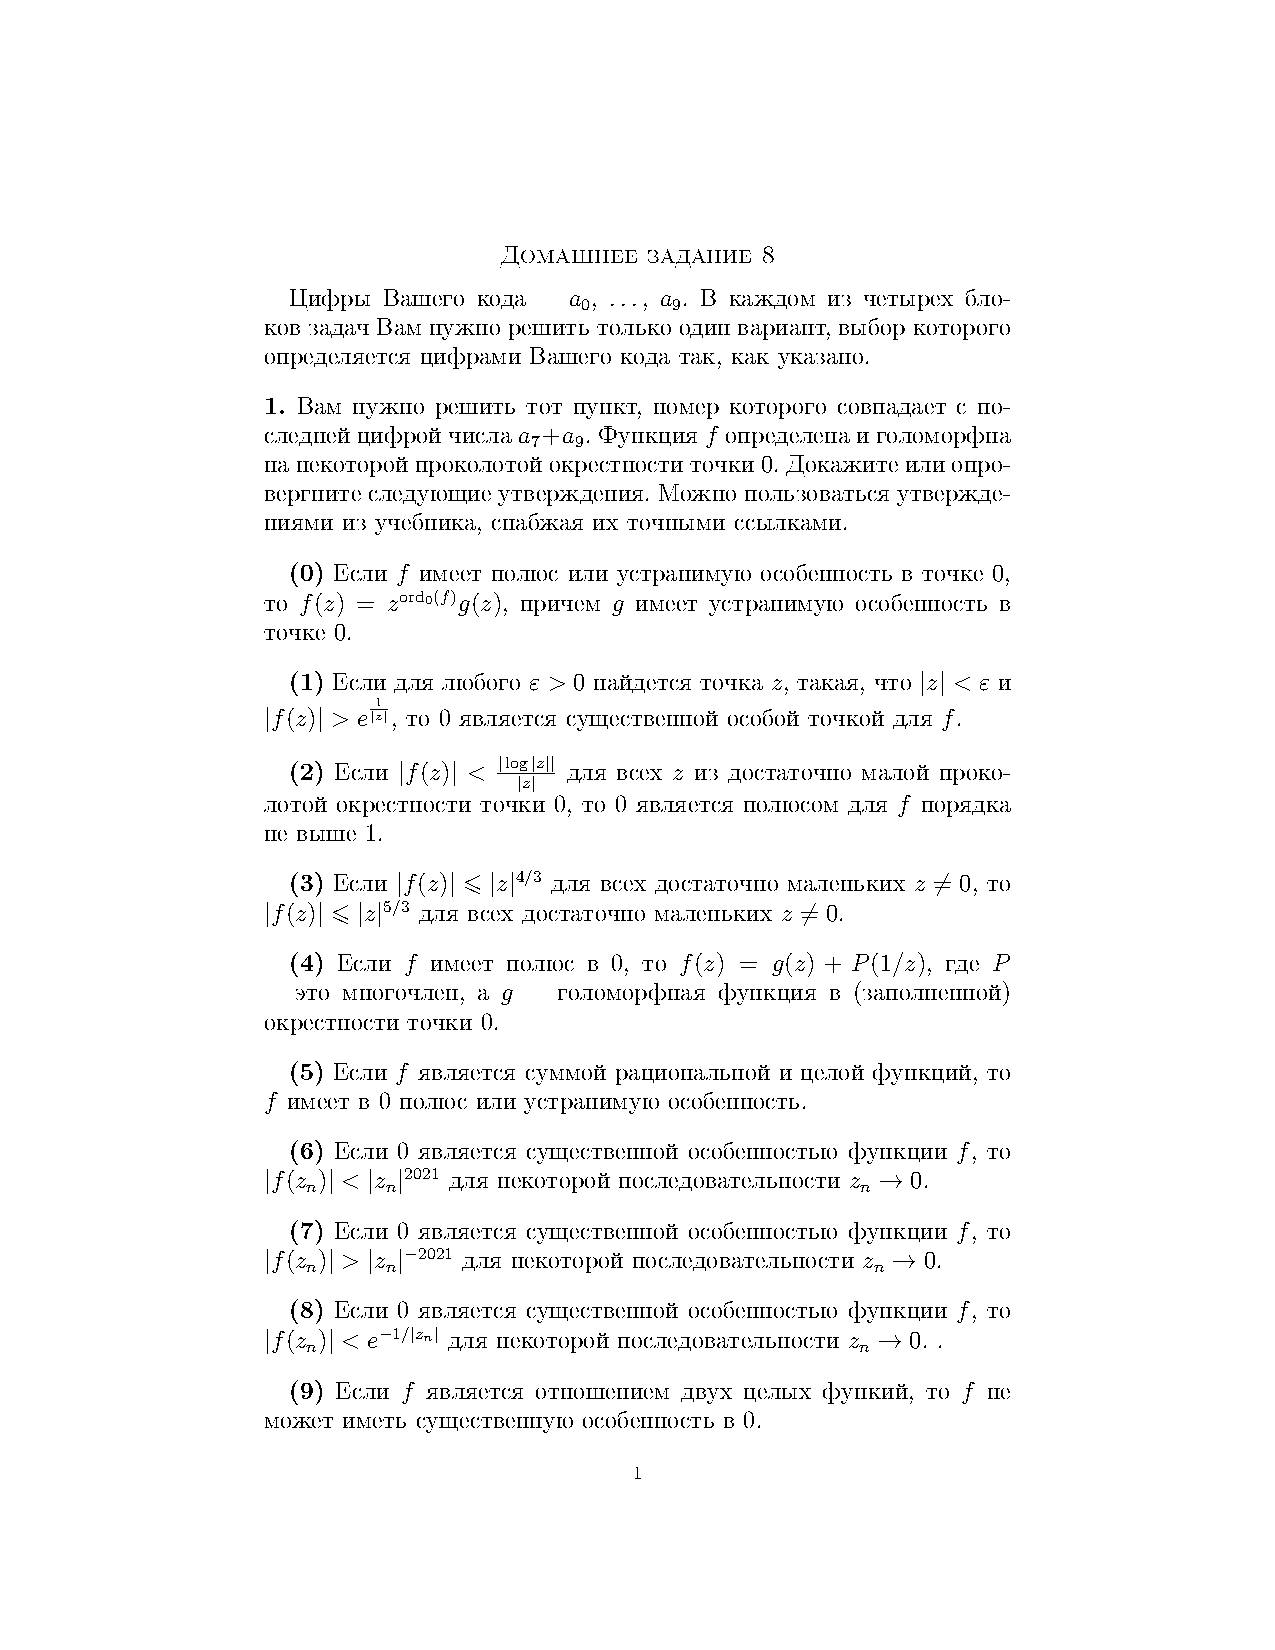
\includepdf[scale=1,pages=1-3]{Tasks/hw8}
\newpage
\section*{Решения}
\subsection*{Задача 1}
	Необходимо решить задачу $a_7 + a_9 = 3 + 6 = 9 \mod 10$
	Пусть $f(z) = \frac{p(z)}{q(z)}$, тогда особенности $f(z)$ это нули $q(z)$ и $\infty$. Так как $q(z)$ -- некий многочлен, то все его нули конечного порядка -- они являются полюсами этого порядка (мы исходим из того, что у $p(z), q(z)$ нет общих корней). Заметим, что $\lim\limits_{z \to \infty} f(z)$ либо $0$ (если $\deg(p) < \deg(q)$), либо $\infty$ (если $\deg(p) > \deg(q)$), либо является отношением коэффициентов перед старшими членами (если $\deg(p) = \deg(q)$), а следовательно предел существует и в $\infty$ также не может быть существенной особенности.\\
	Так мы доказали, что если $f(z)$ является отношением двух целых функций, то у нее вообще нет существуенных особенностей, а следовательно и в 0 они тоже отсутствуют. 
\vskip 0.4in

\subsection*{Задача 2}
	Необходимо решить задачу $a_4 + a_5 = 7 + 6 = 3 \mod 10$
	\begin{gather*}
		\tan(z^3)
	\end{gather*}
	Найдем нули
	\begin{gather*}
		\tan(z^3) = 0\\
		z^3 = \pi n,\ n \in \mathbb{Z}\\
		z_1 = \sqrt[3]{\pi n_1},\ n_1 \in \mathbb{Z}\\
		z_2 = -\frac{1}{2}\sqrt[3]{\pi n_2} + i \frac{\sqrt{3}}{2} \sqrt[3]{\pi n_2},\ n_2 \in \mathbb{Z}\\
		z_3 = -\frac{1}{2}\sqrt[3]{\pi n_3} - i \frac{\sqrt{3}}{2} \sqrt[3]{\pi n_3},\ n_3 \in \mathbb{Z}
	\end{gather*}
	Найдем особенности
	\begin{gather*}
		\tan(z^3)
		= \frac{\sin(z^3)}{\cos(z^3)}
		= - \frac{\cos(z^3 - \frac{\pi}{2})}{\sin(z^3 - \frac{\pi}{2})}
		= \frac{1}{z^3 - \frac{\pi}{2}} \left(-\frac{z^3 - \frac{\pi}{2}}{\sin(z^3 - \frac{\pi}{2})} \cdot \cos(z^3 - \frac{\pi}{2}) \right)
	\end{gather*}
	Уравнение в скобках аналитическое и имеет проколотую окрестность $z^3 = \frac{\pi}{2}$  пределом $-1$ при $z \to \frac{\pi}{2}$, откуда следует что в $z_{1,2,3} = \sqrt[3]{\frac{\pi}{2}}$ полюс порядка 1. Заметим, что другие полюса имеют координаты $z = \sqrt[3]{\frac{(2n+1)\pi}{2}},\ n \in \mathbb{Z}$ (так как $\tan(x) = \tan(\pi + x)$) и также имеют порядок 1.
\vskip 0.4in

\subsection*{Задача 3}
	Необходимо решить задачу $a_5 + a_6 = 6 + 9 = 5 \mod 10$
	\begin{gather*}
		f(z) = \frac{z}{1 + z^3},\ A=\{z \in \mathbb{C}|\ 1 < |z| < \infty\}\\
		\frac{z}{1+z^3}
		= \frac{1}{\frac{1}{z} + z^2}
		= \frac{1}{z^2} \cdot \frac{1}{1 - (-\frac{1}{z^3})}
		= \frac{1}{z^2} \cdot \sum\limits_{n = 0}^{\infty} \left( \left(-\frac{1}{z^3}\right)^n\right)\\
		= \frac{1}{z^2} \cdot \sum\limits_{n = 0}^{\infty} \left( \left(-\frac{1}{z}\right)^{3n}\right)
		= \sum\limits_{n = 0}^{\infty} \left( (-1)^{n}\left(\frac{1}{z}\right)^{3n+2}\right)\\
		\left|\frac{1}{z}\right| < 1
		\Leftrightarrow 1 < |z|
	\end{gather*}
\vskip 0.4in

\subsection*{Задача 4}
	Необходимо решить задачу $a_6 + a_7 = 9 + 3 = 2 \mod 10$
	\begin{gather*}
		f(z) = \frac{e^z}{z^2 - 4}\\
		z = \pm 2
	\end{gather*}
	$\operatorname{Res}_{2}(f)$ равен коэффициенту при $(z - 2)^{-1}$ в разложении $f$ в точке $2$, а $\operatorname{Res}_{-2}(f)$ коэффициенту при $(z + 2)^{-1}$ разложения в точке $-2$.\\
	Разложим в ряд Лорана по степеням $(z - 2)$ в окр $z = 2$
	\begin{gather*}
		\frac{e^z}{z^2 - 4}
		= e^z \cdot \frac{1}{(z - 2)(z + 2)}
		= e^z \cdot \frac{1}{(z - 2)((z - 2) + 4)}
		= e^z \cdot \frac{1}{(z - 2)^2 (1 + \frac{4}{z - 2})}
		= e^z \sum\limits_{k = 0}^{\infty} \frac{(-1)^k 4^k}{(z - 2)^{k+2}}\\
		\operatorname{Res}_{2}(f) = \frac{e^{2}}{-4} = -\frac{e^{2}}{4}
	\end{gather*}
	Разложим в ряд Лорана по степеням $(z + 2)$ в окр $z = -2$
	\begin{gather*}
		\frac{e^z}{z^2 - 4}
		= e^z \cdot \frac{1}{(z - 2)(z + 2)}
		= e^z \cdot \frac{1}{(z + 2)((z + 2) - 4)}
		= e^z \cdot \frac{1}{(z + 2)^2 (1 - \frac{4}{z + 2})}
		= e^z \sum\limits_{k = 0}^{\infty} \frac{(-1)^k 4^k}{(z + 2)^{k+2}}\\
		\operatorname{Res}_{-2}(f) = \frac{e^{-2}}{-4} = -\frac{1}{4e^{2}}
	\end{gather*}
	То есть $\operatorname{Res}_{-2}(f) = -\frac{1}{4e^{2}},\ \operatorname{Res}_{2}(f) = -\frac{e^{2}}{4}$

\begin{comment}
	И тогда
	\begin{gather*}
		\frac{e^z}{z^2 - 4}
		= \frac{e^z}{(z - 2)(z + 2)}
		= \frac{\frac{e^z}{z - 2}}{z + 2}
		= \frac{\frac{e^z}{z - 2}}{z - (-2)}\\
		\operatorname{Res}(f,-2) = \frac{e^{-2}}{-4} = -\frac{1}{4e^{2}}\\
		\operatorname{Res}(f,2) = \frac{e^{2}}{-4} = -\frac{e^{2}}{4}
	\end{gather*}
\end{comment}